\subsection{Comparison with Complete Methods}

\subsubsection{Supervised and Semi-Supervised Recognition}

Table~\ref{tab:full-f0} compares the four complete external methods with the corresponding PAMF recipe. The supervised block uses labeled-only F and same-contract G-L throughout. The semi-supervised block uses each external method with ordinary PL and PAMF-T1 with its native selective self-training, followed by G-LU. PAMF-Sup retains the registered supervised representation objectives and satellite augmentation but consumes no U or EMA; it is not the ordinary-PL control. PAMF-T1 is the fixed final method, not a relabeled PAMF-PL experiment.

\begin{table*}[!t]
\centering\footnotesize
\caption{F0 comparison of complete methods (\%). Raw applies F directly; restored applies the same-contract DURA before F. S6 is the within-seed six-scene mean. Entries are mean$\pm$sample SD over three F seeds.}
\label{tab:full-f0}
\begin{tabular*}{\textwidth}{@{\extracolsep{\fill}}lrrrrr@{}}
\toprule
Method & Raw clean & Raw S6 & Restored clean & Restored S6 & Restored S6 F1 \\
\midrule
\multicolumn{6}{@{}l}{\textit{Supervised F and G-L: labeled source IQ only}} \\
\addlinespace[2pt]
RIEI & \pmv{54.53}{8.31} & \pmv{47.68}{6.42} & \pmv{54.44}{8.24} & \pmv{49.33}{6.36} & \pmv{44.28}{9.42} \\
DRIFT-v2 & \pmv{67.33}{5.91} & \pmv{26.83}{3.36} & \pmv{67.22}{5.96} & \pmv{62.01}{6.30} & \pmv{61.09}{6.55} \\
IB-RFF & \pmv{63.77}{2.18} & \pmv{15.78}{4.87} & \pmv{63.83}{2.18} & \pmv{61.43}{1.98} & \pmv{60.41}{2.27} \\
SDG & \pmv{71.39}{1.84} & \pmv{58.14}{2.32} & \pmv{71.43}{1.85} & \pmv{65.22}{1.85} & \pmv{64.95}{1.49} \\
\textbf{PAMF-Sup} & \pmv{84.01}{0.94} & \pmv{70.08}{1.49} & \pmv{83.95}{0.98} & \pmv{76.84}{0.53} & \pmv{76.49}{0.71} \\
\addlinespace[4pt]
\multicolumn{6}{@{}l}{\textit{Semi-supervised F and G-LU: unlabeled source IQ allowed}} \\
\addlinespace[2pt]
RIEI & \pmv{53.53}{6.48} & \pmv{47.50}{5.66} & \pmv{53.53}{6.49} & \pmv{48.22}{4.86} & \pmv{43.21}{7.89} \\
DRIFT-v2 & \pmv{60.97}{11.26} & \pmv{27.28}{3.11} & \pmv{60.88}{11.31} & \pmv{56.57}{9.42} & \pmv{55.24}{11.36} \\
IB-RFF & \pmv{66.08}{0.99} & \pmv{18.44}{4.30} & \pmv{66.08}{0.96} & \pmv{63.66}{0.96} & \pmv{62.75}{0.63} \\
SDG & \pmv{72.10}{0.41} & \pmv{58.15}{1.53} & \pmv{72.08}{0.41} & \pmv{66.18}{0.21} & \pmv{66.44}{0.35} \\
\textbf{PAMF-T1} & \pmv{84.39}{0.92} & \pmv{70.60}{1.06} & \pmv{84.48}{0.97} & \pmv{77.65}{0.85} & \pmv{77.48}{0.87} \\
\bottomrule
\end{tabular*}
\end{table*}

On F0, PAMF-Sup reaches \pmv{76.84}{0.53}\% S6 accuracy, while PAMF-T1 reaches \pmv{77.65}{0.85}\%. Their respective raw S6 values are \pmv{70.08}{1.49}\% and \pmv{70.60}{1.06}\%. Table~\ref{tab:full-scenes} retains all seven conditions, including the difficult low-urban endpoint. These are complete-recipe comparisons with method-specific objectives and budgets; they do not isolate the effect of an individual SSL component.

\begin{table*}[!t]
\centering\footnotesize
\caption{Restored F0 accuracy on every declared condition (\%). S/U denote suburban/urban and H/M/L denote channel severity. Methods retain the same source and target roles within each setting.}
\label{tab:full-scenes}
\begin{tabular*}{\textwidth}{@{\extracolsep{\fill}}lrrrrrrr@{}}
\toprule
Method & Clean & S-H & S-M & S-L & U-H & U-M & U-L \\
\midrule
\multicolumn{8}{@{}l}{\textit{Supervised: DURA-L}} \\
\addlinespace[2pt]
RIEI & \pmv{54.44}{8.24} & \pmv{52.41}{7.12} & \pmv{51.33}{6.88} & \pmv{50.17}{6.49} & \pmv{51.45}{6.95} & \pmv{47.20}{5.81} & \pmv{43.44}{4.90} \\
DRIFT-v2 & \pmv{67.22}{5.96} & \pmv{65.25}{7.17} & \pmv{64.42}{6.79} & \pmv{63.31}{6.39} & \pmv{64.36}{6.90} & \pmv{59.72}{5.75} & \pmv{55.02}{4.82} \\
IB-RFF & \pmv{63.83}{2.18} & \pmv{63.20}{2.45} & \pmv{62.82}{2.23} & \pmv{62.41}{2.01} & \pmv{62.83}{2.40} & \pmv{60.25}{1.65} & \pmv{57.04}{1.15} \\
SDG & \pmv{71.43}{1.85} & \pmv{69.03}{1.66} & \pmv{67.94}{1.77} & \pmv{66.63}{1.96} & \pmv{67.96}{1.70} & \pmv{62.54}{1.96} & \pmv{57.24}{2.18} \\
\textbf{PAMF-Sup} & \pmv{83.95}{0.98} & \pmv{82.28}{0.76} & \pmv{80.69}{0.57} & \pmv{79.02}{0.51} & \pmv{80.70}{0.66} & \pmv{72.82}{0.45} & \pmv{65.51}{0.47} \\
\addlinespace[4pt]
\multicolumn{8}{@{}l}{\textit{Semi-supervised: DURA-LU}} \\
\addlinespace[2pt]
RIEI & \pmv{53.53}{6.49} & \pmv{50.80}{5.59} & \pmv{49.86}{5.38} & \pmv{48.81}{5.03} & \pmv{49.93}{5.31} & \pmv{46.53}{4.27} & \pmv{43.38}{3.60} \\
DRIFT-v2 & \pmv{60.88}{11.31} & \pmv{59.66}{10.47} & \pmv{58.41}{10.10} & \pmv{56.88}{9.72} & \pmv{59.01}{10.20} & \pmv{54.71}{8.66} & \pmv{50.75}{7.40} \\
IB-RFF & \pmv{66.08}{0.96} & \pmv{65.28}{1.18} & \pmv{64.86}{1.07} & \pmv{64.36}{0.92} & \pmv{65.03}{1.14} & \pmv{62.75}{0.88} & \pmv{59.70}{0.65} \\
SDG & \pmv{72.08}{0.41} & \pmv{70.01}{0.42} & \pmv{68.71}{0.28} & \pmv{67.32}{0.23} & \pmv{68.99}{0.34} & \pmv{63.51}{0.05} & \pmv{58.54}{0.07} \\
\textbf{PAMF-T1} & \pmv{84.48}{0.97} & \pmv{82.30}{0.87} & \pmv{81.00}{0.89} & \pmv{79.47}{0.87} & \pmv{81.06}{0.95} & \pmv{74.40}{0.81} & \pmv{67.66}{0.71} \\
\bottomrule
\end{tabular*}
\end{table*}

\begin{figure*}[!t]\centering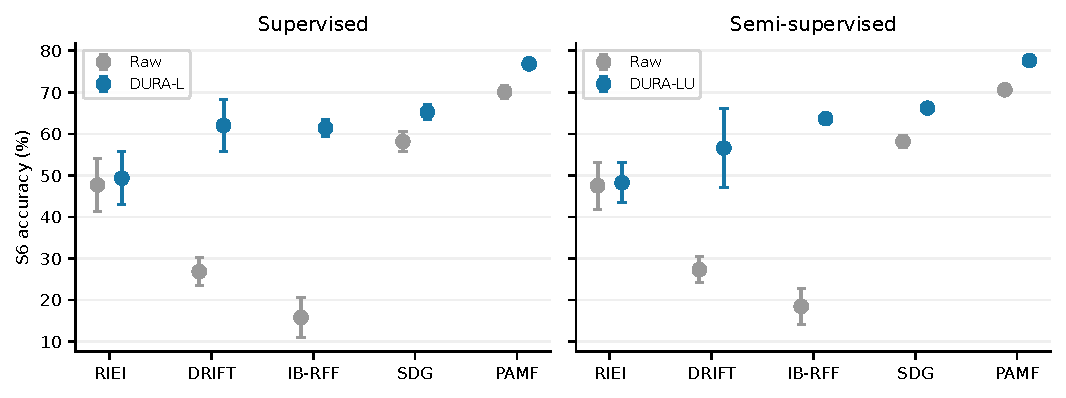
\includegraphics[width=.94\textwidth]{images/full_methods/f0_complete.pdf}\caption{Complete external methods and the corresponding PAMF recipe on F0. Raw and restored S6 accuracy use the same frozen F in each comparison. Error bars are three-F-seed sample SD.}\label{fig:full-f0}\end{figure*}

Restoration does not uniformly improve clean observations or every external classifier. For example, F0 IB-RFF in the supervised setting has S6 accuracy \pmv{61.43}{1.98}\% with G-L, compared with \pmv{15.78}{4.87}\% on raw input; RIEI changes from \pmv{47.68}{6.42}\% to \pmv{49.33}{6.36}\%. All clean reductions and nonmonotonic results remain in the tables and curves. We do not choose the restoration route or bypass from the true test condition.

\subsubsection{Receiver, Date and Label Generalization}

Table~\ref{tab:full-generalization} retains the available complete supervised methods across receiver partitions, the larger TX/RX setting and the future-date endpoint. External semi-supervised models exist for F0 and the natural source-count suite; untrained external SSL cells are not invented for these other conditions. The low-label comparison in Table~\ref{tab:full-labels} includes only the registered IB-RFF and PAMF-Sup models.

\begin{table*}[!t]
\centering\footnotesize
\caption{Supervised generalization with G-L (S6 accuracy, \%). F1/F2 use alternate disjoint RX partitions. ManyRx has ten classes. Chronological evaluation uses target RX on D3 only (42000 packets), not the all-date aggregate.}
\label{tab:full-generalization}
\begin{tabular*}{\textwidth}{@{\extracolsep{\fill}}lrrrr@{}}
\toprule
Method & F1 & F2 & ManyRx & Future D3 \\
\midrule
RIEI & \pmv{56.12}{0.81} & \pmv{59.02}{0.56} & \pmv{26.62}{6.45} & \pmv{52.59}{3.45} \\
DRIFT-v2 & \pmv{56.65}{3.18} & \pmv{61.47}{1.70} & \pmv{40.30}{4.19} & \pmv{60.38}{4.99} \\
IB-RFF & \pmv{58.05}{0.97} & \pmv{60.35}{0.94} & \pmv{62.78}{1.00} & \pmv{68.18}{1.48} \\
SDG & \pmv{59.89}{0.73} & \pmv{64.83}{0.98} & \pmv{64.84}{0.50} & \pmv{70.06}{0.68} \\
\textbf{PAMF-Sup} & \pmv{65.44}{0.36} & \pmv{71.99}{0.63} & \pmv{71.49}{0.33} & \pmv{74.52}{2.36} \\
\bottomrule
\end{tabular*}
\end{table*}

\begin{table}[!t]
\centering\footnotesize
\caption{Label efficiency under full L-only systems (S6 accuracy, \%). Only IB-RFF has registered external low-label models. All rows use the same seven target RX and separate source-validation labels.}
\label{tab:full-labels}
\begin{tabular*}{\columnwidth}{@{\extracolsep{\fill}}lrr@{}}
\toprule
L fraction (\%) & IB-RFF & PAMF-Sup \\
\midrule
1 & \pmv{60.72}{1.49} & \pmv{69.73}{0.46} \\
5 & \pmv{64.05}{1.72} & \pmv{74.29}{0.84} \\
10 & \pmv{61.43}{1.98} & \pmv{76.84}{0.53} \\
\bottomrule
\end{tabular*}
\end{table}

\subsubsection{Source-Receiver Diversity}

Figure~\ref{fig:full-source} compares the five complete methods using exactly six target RX/144000 packets at every point. Natural budgets use $(|L|,|U|,|V|)=(1260m,11340m,5400m)$; the fixed-L/V supervised setting uses $(1080,12600m-1080,5400)$ with no U consumed. The source counts are $m=1,2,3,4,6$. F0 uses seven target RX/168000 packets and is not inserted as an $m=5$ point. A single source RX provides no cross-RX positive pair, so the corresponding PAMF contrast term has zero valid-anchor coverage. Natural SSL curves vary both receiver diversity and available U; they do not isolate receiver count alone.

\begin{figure*}[!t]\centering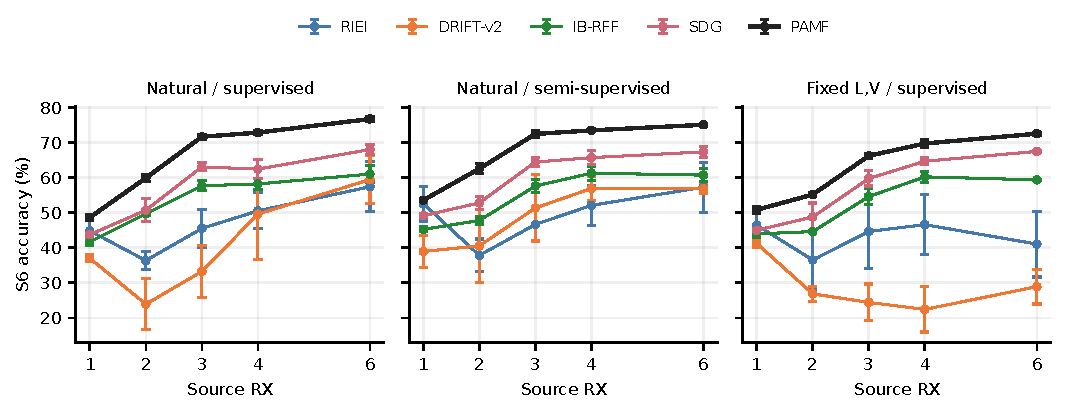
\includegraphics[width=\textwidth]{images/full_methods/source_complete.pdf}\caption{Source-count comparison using complete external methods and PAMF. Supervised panels use G-L; the semi-supervised panel uses G-LU. Each line retains its registered training budget, three F seeds, all negative effects and nonmonotonicity. The fixed-L/V panel controls annotation count.}\label{fig:full-source}\end{figure*}

The source curves provide a broader view than the F0 endpoint: increasing source RX does not guarantee monotonic gains, and PAMF is not assumed to dominate every low-source condition. The source-validation stopping rules remain fixed; test results never select an epoch, branch, seed or rerun.
